\documentclass[]{article}
\usepackage{lmodern}
\usepackage{amssymb,amsmath}
\usepackage{ifxetex,ifluatex}
\usepackage{fixltx2e} % provides \textsubscript
\ifnum 0\ifxetex 1\fi\ifluatex 1\fi=0 % if pdftex
  \usepackage[T1]{fontenc}
  \usepackage[utf8]{inputenc}
\else % if luatex or xelatex
  \ifxetex
    \usepackage{mathspec}
  \else
    \usepackage{fontspec}
  \fi
  \defaultfontfeatures{Ligatures=TeX,Scale=MatchLowercase}
  \newcommand{\euro}{€}
\fi
% use upquote if available, for straight quotes in verbatim environments
\IfFileExists{upquote.sty}{\usepackage{upquote}}{}
% use microtype if available
\IfFileExists{microtype.sty}{%
\usepackage{microtype}
\UseMicrotypeSet[protrusion]{basicmath} % disable protrusion for tt fonts
}{}
\usepackage[margin=1in]{geometry}
\usepackage{hyperref}
\PassOptionsToPackage{usenames,dvipsnames}{color} % color is loaded by hyperref
\hypersetup{unicode=true,
            pdftitle={GCalignR: An R package for aligning Gas-Chromatography data},
            pdfauthor={Meinolf Ottensmann, Martin A. Stoffel, Barbara Casper, Joseph I. Hoffman},
            pdfborder={0 0 0},
            breaklinks=true}
\urlstyle{same}  % don't use monospace font for urls
\usepackage{color}
\usepackage{fancyvrb}
\newcommand{\VerbBar}{|}
\newcommand{\VERB}{\Verb[commandchars=\\\{\}]}
\DefineVerbatimEnvironment{Highlighting}{Verbatim}{commandchars=\\\{\}}
% Add ',fontsize=\small' for more characters per line
\newenvironment{Shaded}{}{}
\newcommand{\KeywordTok}[1]{\textbf{{#1}}}
\newcommand{\DataTypeTok}[1]{\textcolor[rgb]{0.50,0.00,0.00}{{#1}}}
\newcommand{\DecValTok}[1]{\textcolor[rgb]{0.00,0.00,1.00}{{#1}}}
\newcommand{\BaseNTok}[1]{\textcolor[rgb]{0.00,0.00,1.00}{{#1}}}
\newcommand{\FloatTok}[1]{\textcolor[rgb]{0.50,0.00,0.50}{{#1}}}
\newcommand{\ConstantTok}[1]{\textcolor[rgb]{0.00,0.00,0.00}{{#1}}}
\newcommand{\CharTok}[1]{\textcolor[rgb]{1.00,0.00,1.00}{{#1}}}
\newcommand{\SpecialCharTok}[1]{\textcolor[rgb]{1.00,0.00,1.00}{{#1}}}
\newcommand{\StringTok}[1]{\textcolor[rgb]{0.87,0.00,0.00}{{#1}}}
\newcommand{\VerbatimStringTok}[1]{\textcolor[rgb]{0.87,0.00,0.00}{{#1}}}
\newcommand{\SpecialStringTok}[1]{\textcolor[rgb]{0.87,0.00,0.00}{{#1}}}
\newcommand{\ImportTok}[1]{{#1}}
\newcommand{\CommentTok}[1]{\textcolor[rgb]{0.50,0.50,0.50}{\textit{{#1}}}}
\newcommand{\DocumentationTok}[1]{\textcolor[rgb]{0.50,0.50,0.50}{\textit{{#1}}}}
\newcommand{\AnnotationTok}[1]{\textcolor[rgb]{0.50,0.50,0.50}{\textbf{\textit{{#1}}}}}
\newcommand{\CommentVarTok}[1]{\textcolor[rgb]{0.50,0.50,0.50}{\textbf{\textit{{#1}}}}}
\newcommand{\OtherTok}[1]{{#1}}
\newcommand{\FunctionTok}[1]{\textcolor[rgb]{0.00,0.00,0.50}{{#1}}}
\newcommand{\VariableTok}[1]{{#1}}
\newcommand{\ControlFlowTok}[1]{{#1}}
\newcommand{\OperatorTok}[1]{{#1}}
\newcommand{\BuiltInTok}[1]{{#1}}
\newcommand{\ExtensionTok}[1]{{#1}}
\newcommand{\PreprocessorTok}[1]{\textbf{{#1}}}
\newcommand{\AttributeTok}[1]{{#1}}
\newcommand{\RegionMarkerTok}[1]{{#1}}
\newcommand{\InformationTok}[1]{\textcolor[rgb]{0.50,0.50,0.50}{\textbf{\textit{{#1}}}}}
\newcommand{\WarningTok}[1]{\textcolor[rgb]{1.00,0.00,0.00}{\textbf{{#1}}}}
\newcommand{\AlertTok}[1]{\textcolor[rgb]{0.00,1.00,0.00}{\textbf{{#1}}}}
\newcommand{\ErrorTok}[1]{\textcolor[rgb]{1.00,0.00,0.00}{\textbf{{#1}}}}
\newcommand{\NormalTok}[1]{{#1}}
\usepackage{graphicx,grffile}
\makeatletter
\def\maxwidth{\ifdim\Gin@nat@width>\linewidth\linewidth\else\Gin@nat@width\fi}
\def\maxheight{\ifdim\Gin@nat@height>\textheight\textheight\else\Gin@nat@height\fi}
\makeatother
% Scale images if necessary, so that they will not overflow the page
% margins by default, and it is still possible to overwrite the defaults
% using explicit options in \includegraphics[width, height, ...]{}
\setkeys{Gin}{width=\maxwidth,height=\maxheight,keepaspectratio}
\setlength{\parindent}{0pt}
\setlength{\parskip}{6pt plus 2pt minus 1pt}
\setlength{\emergencystretch}{3em}  % prevent overfull lines
\providecommand{\tightlist}{%
  \setlength{\itemsep}{0pt}\setlength{\parskip}{0pt}}
\setcounter{secnumdepth}{5}

%%% Use protect on footnotes to avoid problems with footnotes in titles
\let\rmarkdownfootnote\footnote%
\def\footnote{\protect\rmarkdownfootnote}

%%% Change title format to be more compact
\usepackage{titling}

% Create subtitle command for use in maketitle
\newcommand{\subtitle}[1]{
  \posttitle{
    \begin{center}\large#1\end{center}
    }
}

\setlength{\droptitle}{-2em}
  \title{GCalignR: An R package for aligning Gas-Chromatography data}
  \pretitle{\vspace{\droptitle}\centering\huge}
  \posttitle{\par}
  \author{Meinolf Ottensmann, Martin A. Stoffel, Barbara Casper, Joseph I. Hoffman}
  \preauthor{\centering\large\emph}
  \postauthor{\par}
  \predate{\centering\large\emph}
  \postdate{\par}
  \date{11/1/2015}



% Redefines (sub)paragraphs to behave more like sections
\ifx\paragraph\undefined\else
\let\oldparagraph\paragraph
\renewcommand{\paragraph}[1]{\oldparagraph{#1}\mbox{}}
\fi
\ifx\subparagraph\undefined\else
\let\oldsubparagraph\subparagraph
\renewcommand{\subparagraph}[1]{\oldsubparagraph{#1}\mbox{}}
\fi

\begin{document}
\maketitle

\section{Abstract}\label{abstract}

Key-words: GC-MS, chemical communication, olfactory communication,
alignment

\subsection{Introduction}\label{introduction}

Metabolomics approaches such as Gas Chromatography (GC) and Gas
Chromatography-Mass Spectrometry (GC-MS) are increasingly used by
biologists to unravel the chemical basis of animal olfactory
communication (citations). For the detection of broader patterns in
chemical samples most researchers use an untargeted approach and analyse
the whole spectrum of sampled chemicals rather than targeting specific
compounds. However, chromatography data across multiple samples are not
directly comparable as the retention times of peaks vary across samples
due to subtle, random and often unavoidable variation of the GC-MS
machine parameters (Pierce et al. 2005). For studies that seek to
identify chemical patterns across samples it becomes essential to
account for these retention time drifts by using an appropriate
alignment method.

Despite the existence of automated alignment algorithms (e.g. Smith et
al. 2006; Stein 1999; Robinson et al. 2007) (also gcaligner here), most
researchers in the relatively young fields of mammalian and avian
chemical communication align chromatograms manually (Charpentier,
Boulet, and Drea 2008; Setchell et al. 2010; Caspers et al. 2011;
Leclaire et al. 2012; Theis et al. 2013) or identify all compounds prior
to analysis (Whittaker et al. 2010) rather than using (semi-)automated
alignment software. This approach yields three main drawbacks: (1) For
larger sample sizes, the method is time intensive and can take up to
several weeks. (2) Humans are prone to detect patterns in noise (some
citation) which is why the researcher may bias the alignment due to
subjective experience and expectations. (3) The data analytic pipeline
from the raw GC data to the results of the statistical analysis is not
reproducible.

Here, we introduce \texttt{GCalignR}, a package developed in R, which
provides a simple means of aligning peaks from Gas Chromatography data
and evaluate the quality of the alignment. \texttt{GCalignR} was
specifically developed and tested as a preprocessing tool prior to the
statistical analysis of chemical samples from animal skin and preen
glands (see Stoffel et al. 2015 for an application of the underlying
algorithm). The alignment functions can easily be embedded in
reproducible research tools such as \texttt{Rmarkdown} (citation?) and
piped as input into further statistical packages such as \texttt{vegan}.

\section{The package}\label{the-package}

\paragraph{maybe a flowdiagram (package DiagramR) to illustrate the
complete
workflow}\label{maybe-a-flowdiagram-package-diagramr-to-illustrate-the-complete-workflow}

\begin{enumerate}
\def\labelenumi{\arabic{enumi}.}
\tightlist
\item
  GC / GC-MS analysis
\item
  Peak detection software
\item
  GCalignR workflow
\item
  statistical analysis
\end{enumerate}

\subsection{Data preprocessing}\label{data-preprocessing}

The statistical analysis of GC or GC-MS data is usually based on the
detection of signal peaks within the chromatograms, which is can be done
by proprietary software or free programs such as AMDIS (Stein 1999). The
peak data of a chromatogramm usually contain the retention time of a
given peak plus additional information such as the area under the peak
or its height which are used in the subsequent analysis.
\texttt{GCalignR} aligns peaks via their retention times (and not their
mass-spectra, which may not be available, e.g.~when using
gas-chromatography coupled to a flame ionization detector (FID)) to
align the peaks across individuals for subsequent chemometric analysis
and pattern detection .The simple assumption is that peaks with similar
retention times represent the same substances. However, it is highly
recommended to verify this assumption by comparing also the mass-spectra
(if available) of the substances of interest.

\section{Example dataset}\label{example-dataset}

\paragraph{explanation of example
dataset}\label{explanation-of-example-dataset}

\section{GCalignR workflow}\label{gcalignr-workflow}

\begin{itemize}
\tightlist
\item
  GCalignR steps: Checking the input, aligning chromatograms, evaluating
  alignment
\item
  adjust parameters, align again, evaluate again (if first alignment
  wasn´t satisfactory)
\end{itemize}

\section{Input}\label{input}

\begin{itemize}
\tightlist
\item
  Quickly describe input formats
\item
  Check input and what it checks
\end{itemize}

\begin{Shaded}
\begin{Highlighting}[]
\KeywordTok{check_input}\NormalTok{(}\DataTypeTok{data =} \NormalTok{peak_data,}\DataTypeTok{show_peaks =} \NormalTok{F) }\CommentTok{# If show_peaks = T, a histogram of peaks is plotted }
\CommentTok{#> All checks passed!}
\CommentTok{#> Ready for processing with align_chromatograms}
\end{Highlighting}
\end{Shaded}

\section{Aligning peaks}\label{aligning-peaks}

\begin{itemize}
\tightlist
\item
  describe main features of the main function
\end{itemize}

\begin{Shaded}
\begin{Highlighting}[]
\NormalTok{peak_data_aligned <-}\StringTok{ }\KeywordTok{align_chromatograms}\NormalTok{(}\DataTypeTok{data =} \NormalTok{gc_peak_data, }\CommentTok{# input data}
    \DataTypeTok{conc_col_name =} \StringTok{"area"}\NormalTok{, }\CommentTok{# peak abundance variable}
    \DataTypeTok{rt_col_name =} \StringTok{"time"}\NormalTok{, }\CommentTok{# retention time }
    \DataTypeTok{rt_cutoff_low =} \DecValTok{5}\NormalTok{, }\CommentTok{# cut peaks with retention times below 5 Minutes}
    \DataTypeTok{rt_cutoff_high =} \DecValTok{45}\NormalTok{, }\CommentTok{# cut peaks with retention times above 45 Minutes}
    \DataTypeTok{reference =} \StringTok{"M3"}\NormalTok{, }\CommentTok{# name of reference }
    \DataTypeTok{max_linear_shift =} \FloatTok{0.05}\NormalTok{, }\CommentTok{# maximum linear shift of chromatograms}
    \DataTypeTok{max_diff_peak2mean =} \FloatTok{0.03}\NormalTok{, }\CommentTok{# maximum distance of a peak to the mean}
    \DataTypeTok{min_diff_peak2peak =} \FloatTok{0.03}\NormalTok{, }\CommentTok{# maximum distance between the mean of two peaks}
    \DataTypeTok{blanks =} \OtherTok{NULL}\NormalTok{, }\CommentTok{# no blanks. Specify blanks by names (e.g. c("blank1", "blank2"))}
    \DataTypeTok{delete_single_peak =} \OtherTok{TRUE}\NormalTok{, }\CommentTok{# delete peaks that are present in just one sample }
    \DataTypeTok{write_output =} \OtherTok{NULL}\NormalTok{) }\CommentTok{# add c("time","area") to write data frames to .txt file}
\end{Highlighting}
\end{Shaded}

\begin{Shaded}
\begin{Highlighting}[]
\KeywordTok{data}\NormalTok{(}\StringTok{"aligned_peak_data"}\NormalTok{)}
\end{Highlighting}
\end{Shaded}

\section{Evaluating the quality of the
alignment}\label{evaluating-the-quality-of-the-alignment}

\begin{Shaded}
\begin{Highlighting}[]
\KeywordTok{library}\NormalTok{(ggplot2)}
\KeywordTok{library}\NormalTok{(gridExtra)}
\end{Highlighting}
\end{Shaded}

\begin{Shaded}
\begin{Highlighting}[]
\KeywordTok{gc_heatmap}\NormalTok{(aligned_peak_data,}\DataTypeTok{threshold =} \FloatTok{0.01}\NormalTok{, }\DataTypeTok{samples_subset =} \DecValTok{1}\NormalTok{:}\DecValTok{20}\NormalTok{, }\DataTypeTok{substance_subset =} \DecValTok{1}\NormalTok{:}\DecValTok{30}\NormalTok{, }\DataTypeTok{label_size =} \DecValTok{10}\NormalTok{) }\CommentTok{# By default a threshold of 0.05 is used to mark deviations}
\end{Highlighting}
\end{Shaded}

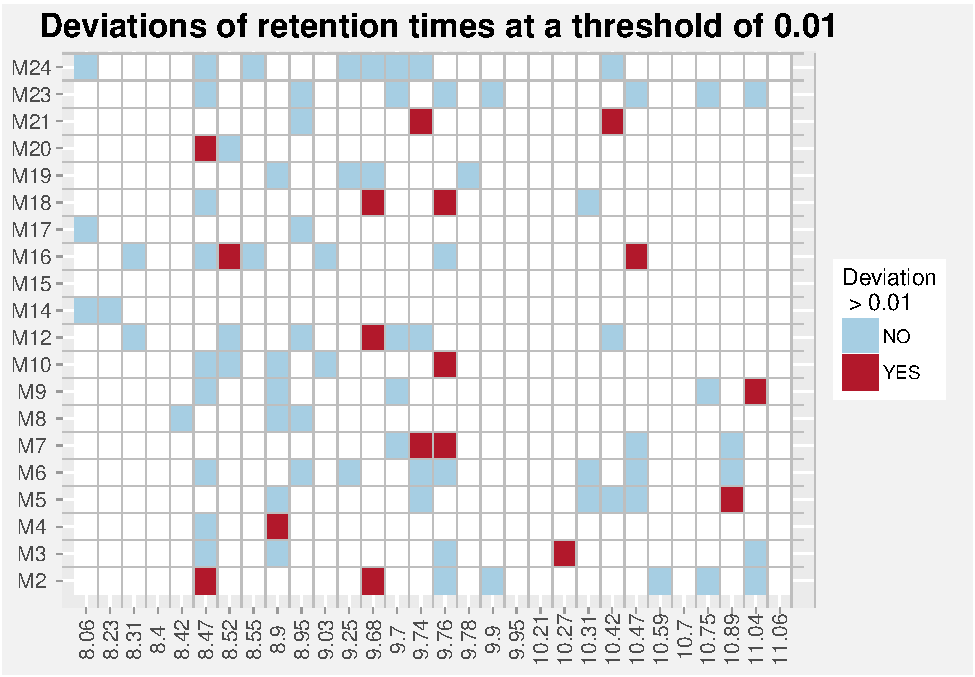
\includegraphics{GCalignR_paper_files/figure-latex/unnamed-chunk-8-1.pdf}

\subsection{Availability}\label{availability}

The latest version of \texttt{GCalignR} can be downloaded from GitHub.

\begin{Shaded}
\begin{Highlighting}[]
\KeywordTok{install.packages}\NormalTok{(}\StringTok{"devtools"}\NormalTok{)}
\NormalTok{devtools::}\KeywordTok{install_github}\NormalTok{(}\StringTok{"mastoffel/GCalignR"}\NormalTok{)}
\end{Highlighting}
\end{Shaded}

We welcome any contributions or feedback on the package.

\subsection{Data accessibility}\label{data-accessibility}

\subsection*{References}\label{references}
\addcontentsline{toc}{subsection}{References}

\hypertarget{refs}{}
\hypertarget{ref-caspers2011scents}{}
Caspers, Barbara A, Frank C Schroeder, Stephan Franke, and Christian C
Voigt. 2011. ``Scents of Adolescence: The Maturation of the Olfactory
Phenotype in a Free-Ranging Mammal.'' \emph{PloS One} 6 (6). Public
Library of Science: e21162.

\hypertarget{ref-charpentier2008smelling}{}
Charpentier, Marie JE, MarylENe Boulet, and Christine M Drea. 2008.
``Smelling Right: The Scent of Male Lemurs Advertises Genetic Quality
and Relatedness.'' \emph{Molecular Ecology} 17 (14). Wiley Online
Library: 3225--33.

\hypertarget{ref-leclaire2012semiochemical}{}
Leclaire, Sarah, Thomas Merkling, Christine Raynaud, Hervé Mulard,
Jean-Marie Bessière, Émeline Lhuillier, Scott A Hatch, and Étienne
Danchin. 2012. ``Semiochemical Compounds of Preen Secretion Reflect
Genetic Make-up in a Seabird Species.'' \emph{Proceedings of the Royal
Society of London B: Biological Sciences} 279 (1731). The Royal Society:
1185--93.

\hypertarget{ref-pierce2005classification}{}
Pierce, Karisa M, Janiece L Hope, Kevin J Johnson, Bob W Wright, and
Robert E Synovec. 2005. ``Classification of Gasoline Data Obtained by
Gas Chromatography Using a Piecewise Alignment Algorithm Combined with
Feature Selection and Principal Component Analysis.'' \emph{Journal of
Chromatography A} 1096 (1). Elsevier: 101--10.

\hypertarget{ref-robinson2007dynamic}{}
Robinson, Mark D, David P De Souza, Woon W Keen, Eleanor C Saunders,
Malcolm J McConville, Terence P Speed, and Vladimir A Likić. 2007. ``A
Dynamic Programming Approach for the Alignment of Signal Peaks in
Multiple Gas Chromatography-Mass Spectrometry Experiments.'' \emph{BMC
Bioinformatics} 8 (1). BioMed Central Ltd: 419.

\hypertarget{ref-setchell2010odour}{}
Setchell, Joanna M, Stefano Vaglio, Kristin M Abbott, Jacopo
Moggi-Cecchi, Francesca Boscaro, Giuseppe Pieraccini, and Leslie A
Knapp. 2010. ``Odour Signals Major Histocompatibility Complex Genotype
in an Old World Monkey.'' \emph{Proceedings of the Royal Society of
London B: Biological Sciences}. The Royal Society, rspb20100571.

\hypertarget{ref-smith2006xcms}{}
Smith, Colin A, Elizabeth J Want, Grace O'Maille, Ruben Abagyan, and
Gary Siuzdak. 2006. ``XCMS: Processing Mass Spectrometry Data for
Metabolite Profiling Using Nonlinear Peak Alignment, Matching, and
Identification.'' \emph{Analytical Chemistry} 78 (3). ACS Publications:
779--87.

\hypertarget{ref-stein1999integrated}{}
Stein, Stephen E. 1999. ``An Integrated Method for Spectrum Extraction
and Compound Identification from Gas Chromatography/mass Spectrometry
Data.'' \emph{Journal of the American Society for Mass Spectrometry} 10
(8). Elsevier: 770--81.

\hypertarget{ref-stoffel2015chemical}{}
Stoffel, Martin A, Barbara A Caspers, Jaume Forcada, Athina Giannakara,
Markus Baier, Luke Eberhart-Phillips, Caroline Müller, and Joseph I
Hoffman. 2015. ``Chemical Fingerprints Encode Mother--offspring
Similarity, Colony Membership, Relatedness, and Genetic Quality in Fur
Seals.'' \emph{Proceedings of the National Academy of Sciences} 112
(36). National Acad Sciences: E5005--E5012.

\hypertarget{ref-theis2013symbiotic}{}
Theis, Kevin R, Arvind Venkataraman, Jacquelyn A Dycus, Keith D Koonter,
Emily N Schmitt-Matzen, Aaron P Wagner, Kay E Holekamp, and Thomas M
Schmidt. 2013. ``Symbiotic Bacteria Appear to Mediate Hyena Social
Odors.'' \emph{Proceedings of the National Academy of Sciences} 110
(49). National Acad Sciences: 19832--7.

\hypertarget{ref-whittaker2010songbird}{}
Whittaker, Danielle J, Helena A Soini, Jonathan W Atwell, Craig Hollars,
Milos V Novotny, and Ellen D Ketterson. 2010. ``Songbird Chemosignals:
Volatile Compounds in Preen Gland Secretions Vary Among Individuals,
Sexes, and Populations.'' \emph{Behavioral Ecology} 21 (3). ISBE:
608--14.

\end{document}
